\documentclass{../../ece-report}

\usepackage{subcaption}

\memostudent{Ty Davis}
\memotitle{Lab 3 - Diode Based Limiting and Clamping Circuits}
\memocourse{ECE 3110}
\memodate{\today}

\newcommand{\twosubfigures}[6]{
  \begin{subfigure}{0.45\textwidth}
    \includegraphics[width=\textwidth]{#1}
    \caption{#2}
    \label{#3}
  \end{subfigure}
  \begin{subfigure}{0.45\textwidth}
    \includegraphics[width=\textwidth]{#4}
    \caption{#5}
    \label{#6}
  \end{subfigure}
}

\begin{document}

\maketitle

\section{Introduction}

In this report we analyze the circuits shown in Fig.~\ref{fig:ciruits}
through computer simulation, then compare the results
with measurements we record in the lab with the oscilloscope.
All of these circuits are commonly used diode circuits
and will produce unique outputs.

\begin{figure}[h!]
  \centering
  \begin{subfigure}{.45\textwidth}
    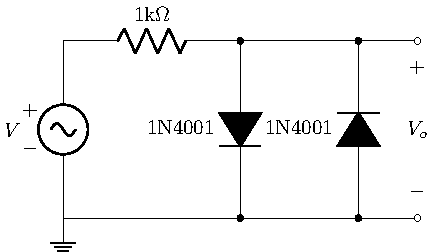
\includegraphics[width=\textwidth]{../circuits/circuit_a.pdf}
    \caption{Limiter Circuit}
    \label{fig:circuit_a}
  \end{subfigure}
  \begin{subfigure}{.45\textwidth}
    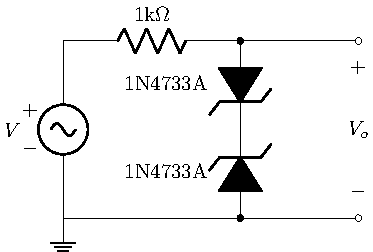
\includegraphics[width=\textwidth]{../circuits/circuit_b.pdf}
    \caption{Zener Diode Limiter Circuit}
    \label{fig:circuit_b}
  \end{subfigure}
  \begin{subfigure}{.45\textwidth}
    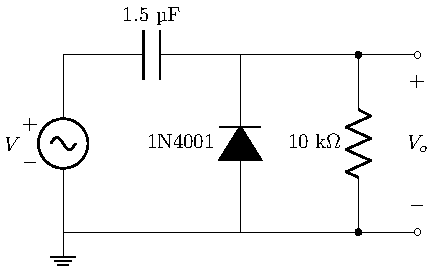
\includegraphics[width=\textwidth]{../circuits/circuit_c.pdf}
    \caption{Clamping Circuit}
    \label{fig:circuit_c}
  \end{subfigure}
  \begin{subfigure}{.45\textwidth}
    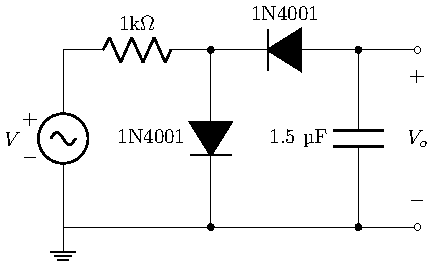
\includegraphics[width=\textwidth]{../circuits/circuit_d.pdf}
    \caption{Voltage Doubler Circuit}
    \label{fig:circuit_d}
  \end{subfigure}
  \caption{Circuits That are Used in This Lab}
  \label{fig:ciruits}
\end{figure}

\section{Limiter Circuits}

Limiter circuits are used to limit the output of an
input wave. They often appear linear until some certain
voltage threshold where they cut off and almost stop
increasing entirely.

The limiter circuit shown in Fig.~\ref{fig:circuit_a}
is a circuit that uses the voltage drop over a single
1N4001 diode to limit the output voltage of the circuit.
Because the voltage increase is extremely low for any
extreme increase in current, the voltage over the diode
peaks at around 0.6~\si{\V}. The function works by acting
linear, essentially just a voltage passing through a
resistor, when neither of the diodes are turned on.
Though, when one of the diodes becomes forward biased,
it acts as a short circuit and only the voltage drop
across the diode is seen at the output.

By placing two diodes in parallel and facing opposite
directions, the circuit doesn't limit only when the
voltage is positive (or negative). Rather, the circuit
is able to allow current to pass through the diodes
in either case, and the voltage is seen on the output
whether the input voltage is positive or negative.

To increase the limiting voltage to 1.4~\si{\V}, all that
we needed to do was place another diode in series with
each of the two diodes. This made the voltage drop across the 
network equal to 2 times the original voltage drop, and it 
was very close 1.4~\si{\V}.

In Fig.~\ref{fig:limiter_results} you can see the voltage
of the output graphed with respect to the input in both
the simulation and the experiment. Clearly, the behavior
was modeled well and the circuit behaves as expected.


\begin{figure}[h!]
  \centering
  \twosubfigures{../plots/circuit_a/pdf/a_sim_xy.pdf}{Simulated}{fig:a_simulated}
                {../plots/circuit_a/pdf/a_meas_xy.pdf}{Measured}{fig:a_measured}
  \caption{Limiter Circuit Simulation and Measurements}
  \label{fig:limiter_results}
\end{figure}

Similar to the normal diode limiter circuit, Zener diodes
(see Fig.~\ref{fig:circuit_b}) can be utilized to specify
the target voltage that the input will be limited to.
The Zener diodes that we chose (1N4733A) become forward
biased at around 5~\si{\V}, and as such the output voltage
is limited to that value. See Fig.~\ref{fig:zener_limiter_results}
to compare the simulated vs measured results of the
Zener diode limiter.

\begin{figure}[h!]
  \centering
  \twosubfigures{../plots/circuit_b/pdf/b_sim_xy.pdf}{Simulated}{fig:b_simulated}
                {../plots/circuit_b/pdf/b_meas_xy.pdf}{Measured}{fig:b_measured}
  \caption{Zener Diode Limiter Circuit Simulation and Measurements}
  \label{fig:zener_limiter_results}
\end{figure}

\section{Clamping Circuit}

A clamper circuit is used to translate some input voltage
to either a completely positive voltage or a completely
negative voltage. The circuit works by charging the
capacitor when the input voltage is negative and the
diode is forward biased, and when the input voltage
is positive the diode is reverse biased and as such
doesn't allow current to flow, so the output is just
the input voltage plus whatever the capacitor was charged
to while the input was negative. 

Assuming an ideal diode, the output voltage of the circuit
would be exactly equal to the input voltage shifted
until it all becomes positive. Of course, because of
the non-zero voltage drop over the resistor, this isn't
exactly the case, but the circuit still reaches a nearly
all-positive state, within the voltage drop of the diode.

In the simulation, as shown in Fig.~\ref{fig:c_simulated},
we can see that the output voltage is higher than in
the experimental measurement. This is because we did
not wait in the simulation for long enough so that the
circuit could find a consistent state. The capacitor
was still charged more than it would be several iterations
past this point. Given enough time that the simulated
circuit could reach some form of equilibrium, it is
anticipated that it would appear very similar to the
measured results, which were captured after the circuit
had ample time to settle.

\begin{figure}[h!]
  \centering
  \twosubfigures{../plots/circuit_c/pdf/c_sim_trans.pdf}{Simulated}{fig:c_simulated}
                {../plots/circuit_c/pdf/c_meas_trans.pdf}{Measured}{fig:c_measured}
  \caption{Limiter Circuit Simulation and Measurements}
  \label{fig:clamped_results}
\end{figure}

By changing the direction of the diode and having it
face backwards, the voltage of the output voltage of
the circuit is clamped the other way and the voltage
moves to be completely negative, or with real components
the output voltage is clamped to less than 0.5~\si{\V}.
See Fig.~\ref{fig:negative_clamped_results}.

\begin{figure}[h!]
  \centering
  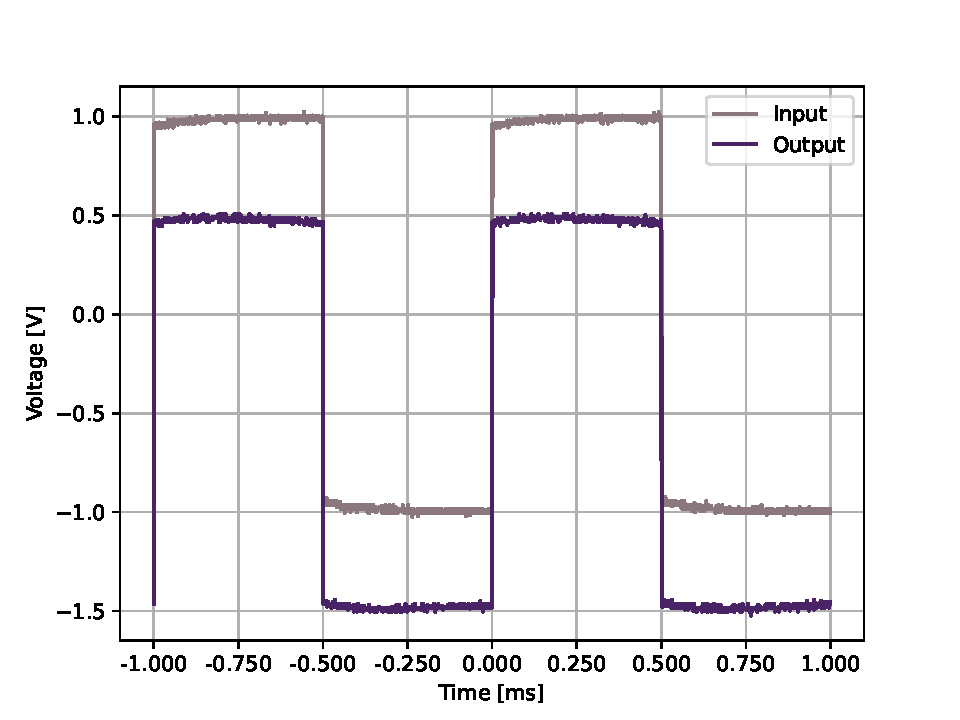
\includegraphics[width=0.45\textwidth]{../plots/circuit_c/pdf/c_meas_-0_7.pdf}
  \caption{Negative clamping circuit measurement}
  \label{fig:negative_clamped_results}
\end{figure}


\section{Voltage Doubler Circuit}

The voltage doubler is essentially a peak rectifier
circuit with a configuration of diodes that allows a
capacitor to feed into itself alongside the voltage
source. The result of passing in an AC voltage is essentially
a DC voltage output that is just larger than 2 times
the RMS voltage of the input, with a very slight ripple.
Refer to Fig.~\ref{fig:doubler_results} to see the simulated
and experimental results.

\begin{figure}[h!]
  \centering
  \twosubfigures{../plots/circuit_d/pdf/d_sim_trans.pdf }{Simulated}{fig:d_simulated}
                {../plots/circuit_d/pdf/d_meas_trans.pdf}{Measured}{fig:d_measured}
  \caption{Limiter Circuit Simulation and Measurements}
  \label{fig:doubler_results}
\end{figure}

\section{Conclusion}

After reviewing these circuits, we found that the expected
behavior of all the circuits was very similar to our
simulation results. Allowing the clamper circuit simulation
to settle a bit longer before grabbing the results would
have likely resulted in our numbers lining up just a
bit better, but regardless our simulations and experimental
measurements were consistent. Personally, I find developing
an intuition for some of these circuits a little bit
difficult, especially the clamper and doubler circuits,
but practice in the lab aids in learning how all of
these circuits function.

\end{document}
